\def\SigleNumero{STT-1900}
\def\NomCours{Méthodes statistiques pour l'ingénierie}
\def\DateEvaluation{22 mars 2026}
\def\HeureEvaluation{13h30 à 16h20}
\def\Session{}
\def\NomEvaluation{Examen de reprise 1}
\def\Ponderation{45}
% Ne rien mettre entre les accolades si l'enseignant (ou l'enseignante) est aussi le coordonnateur (ou la coordonnatrice)
\def\Coordonnatrice{}
\def\Coordonnateur{}

% Ne rien mettre entre les accolades s'il y a plus d'une section
\def\Enseignant{Julien Miron}
\def\Enseignante{}

% Ne rien mettre entre les accolades s'il s'agit d'un cours à section unique
% Mettre le nom de chacun des enseignants et enseignantes entre les accolades
% Une case à cocher sera générée pour chacune des sections
\def\SectionA{}
\def\SectionB{}
\def\SectionC{}
\def\SectionD{}

\newcommand{\affichepoints}{}     % ← AVEC points
% \renewcommand{\affichepoints}{on} % ← SANS points (non vide)

\def\Directives{
\begin{enumerate}
\item Matériel autorisé:
\begin{itemize}
\item Calculatrice scientifique {\bf autorisée par la faculté des sciences et de génie};
\item Votre aide-mémoire d'une feuille recto-verso, écrit à la main.
\end{itemize}
\item Assurez-vous que cette évaluation comporte \numquestions ~exercices répartis sur \numpages{}~pages, pour un total de \numpoints{}~points.\
\item \textbf{Veuillez ne pas dégrafer votre examen.}
\item Vous devez\textbf{ justifier toutes vos réponses} par une démarche claire, sauf pour les questions à choix de réponse.\
\item Pour les questions à choix de réponse et les vrais ou faux, vous pouvez mettre un X, un crochet ($\checkmark$) ou remplir la case.\
\item Vous devez laisser tout ce qui ne servira pas durant l'examen à l'avant de la salle AVANT de rejoindre votre place.\
\item Vous n'avez droit à AUCUN appareil électronique en votre possession durant l'examen.
\item Une fois assis à votre place, vous devez demandez l'autorisation pour vous lever, même si l'examen n'est pas encore commencé.
\item Dans les 5 dernières minutes de l'examen, il sera interdit de se lever avant que TOUTES les copies n'aient été ramassées.
\end{enumerate}
\begin{itemize}
\item[$\rightarrow$] Le non-respect des consignes 7-8-9 entraînera une pénalité de 10\%.
\end{itemize}
}



\documentclass{Evaluation}
\usepackage{multicol,graphicx}

\printanswers

\begin{document}

\pageblanche
%%%%%%%%%%%%%%%% QUESTION %%%%%%%%%%%%%%%%
\begin{questions}
\question[3] Soit l'histogramme ci-dessous. \\



\begin{center}

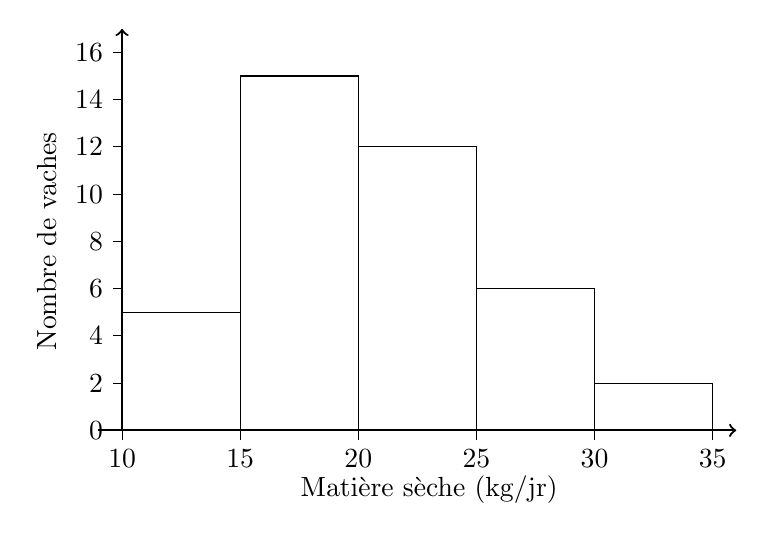
\begin{tikzpicture}[x=0.3cm,y=0.3cm]

% -------------------------------------------------
% Axes
% -------------------------------------------------
\draw[->, thick] (9,0) -- (36,0);   % axe x
\draw[->, thick] (10,0) -- (10,17); % axe y

% -------------------------------------------------
% Graduations x
% -------------------------------------------------
\foreach \x in {10,15,20,25,30,35}
  \draw (\x,0) -- (\x,-0.4) node[below] {\x};

% -------------------------------------------------
% Graduations y
% -------------------------------------------------
\foreach \y in {0,2,4,6,8,10,12,14,16}
  \draw (10,\y) -- (9.6,\y) node[left] {\y};

% -------------------------------------------------
% Labels
% -------------------------------------------------
\node at (23,-2.5) {Matière sèche (kg/jr)};
\node[rotate=90] at (6.8,8) {Nombre de vaches};

% -------------------------------------------------
% Histogramme (rectangles)
% Classes : [10,15[, [15,20[, [20,25[, [25,30[, [30,35[
% Effectifs : 5, 15, 12, 6, 2
% -------------------------------------------------
\draw (10,0) rectangle (15,5);
\draw (15,0) rectangle (20,15);
\draw (20,0) rectangle (25,12);
\draw (25,0) rectangle (30,6);
\draw (30,0) rectangle (35,2);

\end{tikzpicture}
\end{center}


Dans quelle classe de l'histogramme se situe le quantile d'ordre 0,60?

	\begin{checkboxes}
		\choice Dans la classe [10,15[
		\choice Dans la classe [15,20[
		\correctchoice Dans la classe [20,25[
		\choice Dans la classe [25,30[
		\choice Dans la classe [30,35]
	\end{checkboxes}

\begin{solution}
    Le nombre total de vaches est $5+15+12+6+2=40$. Le quantile d'ordre $0{,}60$ correspond à la position $0{,}60 \times 40 = 24$. L'effectif cumulé après la classe $[10,15[$ est $5$. L'effectif cumulé après la classe $[15,20[$ est $5+15=20$. L'effectif cumulé après la classe $[20,25[$ est $20+12=32$. Puisque $20 < 24 \leq 32$, le quantile d'ordre $0{,}60$ se situe dans la classe $[20,25[$.
\end{solution}

\vspace{0.3cm}

\question[] Dites si chaque énoncé est vrai ou faux.

\begin{parts}
    \part[1] Si $A$ et $B$ sont deux événements mutuellement exclusifs, alors $P(A \cup B) = P(A) + P(B)$.
    \begin{oneparcheckboxes}
        \correctchoice Vrai
        \choice Faux
    \end{oneparcheckboxes}

    \begin{solution}
        Vrai. C'est la propriété d'additivité: si $A \cap B = \emptyset$, alors $P(A \cup B) = P(A) + P(B)$.
    \end{solution}

    \part[1] Si $P(A) = 0{,}6$ et $P(B) = 0{,}5$, alors $A$ et $B$ peuvent être mutuellement exclusifs.

        \begin{oneparcheckboxes}
        \choice Vrai
        \correctchoice Faux
    \end{oneparcheckboxes}

    \begin{solution}
        Faux. Si $A$ et $B$ étaient mutuellement exclusifs, on aurait $P(A \cup B) = P(A) + P(B) = 0{,}6 + 0{,}5 = 1{,}1 > 1$, ce qui est impossible.
    \end{solution}

        \part[1] Si $A$ et $B$ sont deux événements indépendants, alors $P(A \cap B) = 0$.

        \begin{oneparcheckboxes}
        \choice Vrai
        \correctchoice Faux
    \end{oneparcheckboxes}

    \begin{solution}
        Faux. Si $A$ et $B$ sont indépendants, on a $P(A \cap B) = P(A) \cdot P(B)$, qui n'est pas nécessairement $0$ (sauf si $P(A)=0$ ou $P(B)=0$).
    \end{solution}

        \part[1] Si $P(A \cup B) = 1$, alors $A$ et $B$ sont complémentaires.

        \begin{oneparcheckboxes}
        \choice Vrai
        \correctchoice Faux
    \end{oneparcheckboxes}

    \begin{solution}
        Faux. On peut avoir $P(A \cup B) = 1$ sans que $A$ et $B$ soient complémentaires. Par exemple, $P(A)=0{,}8$, $P(B)=0{,}5$ et $P(A\cap B)=0{,}3$ donnent $P(A \cup B)=1$, mais $B \neq A^c$.
    \end{solution}
\end{parts}


\vspace{0.3cm}
\question On a mesuré le temps de réaction (en millisecondes) de seize étudiants. 
L'intervalle de confiance à 95\% obtenu pour le temps de réaction moyen est $[42; 54]$.
On suppose que la loi normale est adéquate pour cette variable aléatoire.


\begin{parts}
\part[1] On a confiance à 95\% que cet intervalle contient la vraie valeur moyenne du temps de réaction. 

\begin{oneparcheckboxes}
    \correctchoice Vrai
    \choice Faux
\end{oneparcheckboxes}

\begin{solution}
    Vrai. C'est l'interprétation correcte d'un intervalle de confiance: on a confiance au niveau 95\% que l'intervalle construit contient la vraie valeur du paramètre $\mu$.
\end{solution}

    \part[1] Le temps de réaction moyen des étudiants ayant participé à l'étude est de 50 millisecondes.
    
    \begin{oneparcheckboxes}
        \choice Vrai
        \correctchoice Faux
    \end{oneparcheckboxes}

    \begin{solution}
        Faux. L'intervalle de confiance est symétrique autour de $\bar{x}$. Donc $\bar{x}=(42+54)/2=48$, et non $50$.
    \end{solution}

    \part[1] Si on recommençait la même expérience avec seize autres individus de la même population, il y aurait 95\% de chances que la nouvelle moyenne échantillonnale soit comprise entre 42 et 54.
    
    \begin{oneparcheckboxes}
        \choice Vrai
        \correctchoice Faux
    \end{oneparcheckboxes}

    \begin{solution}
        Faux. L'intervalle de confiance ne prédit pas la valeur d'une future moyenne échantillonnale. Le niveau de confiance de 95\% signifie que la procédure de construction de l'intervalle capture $\mu$ dans 95\% des cas.
    \end{solution}

    \part[1] Environ 95\% des étudiants de cette population ont un temps de réaction compris entre 42 et 54.
    
    \begin{oneparcheckboxes}
        \choice Vrai
        \correctchoice Faux
    \end{oneparcheckboxes}

    \begin{solution}
        Faux. L'intervalle de confiance est construit pour la moyenne $\mu$, pas pour les valeurs individuelles de la population.
    \end{solution}

        \part[1] Environ 95\% des étudiants de cet échantillon ont un temps de réaction compris entre 42 et 54.
    
    \begin{oneparcheckboxes}
        \choice Vrai
        \correctchoice Faux
    \end{oneparcheckboxes}

    \begin{solution}
        Faux. L'intervalle de confiance ne porte pas sur la proportion d'individus de l'échantillon dans un intervalle, mais bien sur la localisation de la moyenne $\mu$.
    \end{solution}
    
\end{parts}

\pageblanche
\question Un sac contient 30 dés rouges, 50 dés verts et 20 dés bleus.
Les dés rouges et les dés verts sont numérotés de <<1>> à <<6>>.
Les dés bleus ont 6 fois la face <<6>>.

L'expérience aléatoire consiste à choisir un dé dans le sac, à le lancer et à noter la face du dessus.

Pour répondre aux questions, utilisez $\mathcal{S}$ pour désigner l'espace échantillonnal et les événements suivants:

\begin{itemize}
    \item R: le dé choisi est rouge,
    \item V: le dé choisi est vert,
    \item B: le dé choisi est bleu,
    \item S: la face sur le dessus du dé lancé est <<6>>,
    \item D: la face sur le dessus du dé lancé est <<2>>.
\end{itemize}

\begin{parts}
    \part[7] La face sur le dessus du dé lancé est <<6>>. Quelle est la probabilité que le dé lancé soit bleu?


\begin{solution}
    On sait que $P(R)=0{,}3$, $P(V)=0{,}5$, $P(B)=0{,}2$, $P(S|R)=P(S|V)=\sfrac{1}{6}$, $P(S|B)=1$. On peut déduire que 

    \begin{align*}
        P(S)&=P(S\cap R)+P(S\cap V)+P(S\cap B)\\
        &= P(S|R)P(R)+P(S|V)P(V)+P(S|B)P(B)\\
        &=\frac{1}{6}\times 0{,}3+\frac{1}{6}\times 0{,}5 + 1 \times 0{,}2\\
        &=\frac{0{,}8}{6}+0{,}2\\
        &=\frac{4}{30}+\frac{6}{30}\\
        &=\displaystyle\frac{1}{3}
    \end{align*}

    On cherche $P(B|S)$.

    \begin{align*}
        P(B|S)&=\frac{P(S\cap B)}{P(S)}\\
        &=\frac{P(S|B)P(B)}{P(S)}\\
        &= \frac{1\times 0{,}2}{\sfrac{1}{3}}\\
        &=\frac{3}{5}
    \end{align*}
\end{solution}

\vfill

\part[3] Quel énoncé est vrai parmi les suivants?

\begin{checkboxes}
    \choice Les événements $R$ et $B$ sont indépendants.
    \correctchoice Les événements $R$ et $B$ sont mutuellement exclusifs.
    \choice Les événements $B$ et $S$ sont indépendants.
    \choice Les événements $B$ et $S$ sont mutuellement exclusifs.
\end{checkboxes}

\begin{solution}
    \begin{itemize}
        \item $R$ et $B$ ne sont pas indépendants car $P(R \cap B)=0 \neq P(R)P(B)=0{,}3\times0{,}2=0{,}06$.
        \item $R$ et $B$ sont mutuellement exclusifs car un dé ne peut pas être à la fois rouge et bleu, donc $P(R \cap B)=0$.
        \item $B$ et $S$ ne sont pas indépendants car $P(B \cap S)=P(S|B)P(B)=1\times 0{,}2=0{,}2$ alors que $P(B)P(S)=0{,}2\times\sfrac{1}{3}=\sfrac{1}{15}\neq 0{,}2$.
        \item $B$ et $S$ ne sont pas mutuellement exclusifs car $P(B \cap S)=0{,}2\neq 0$.
    \end{itemize}
\end{solution}

\end{parts}


\pageblanche

\question\label{densite} Soit $X$ une variable aléatoire continue de densité $f_X$ définie ci-dessous.

\begin{minipage}[]{7cm}{
\vspace{0cm}
\[ f_X(x) = \begin{cases}
\vspace{0.2cm}
\displaystyle \frac{1}{14} & \mbox{si } 0\leq x < \displaystyle \frac{a}{4}, \\
\vspace{0.2cm}
\displaystyle \frac{1}{7} & \mbox{si } \displaystyle\frac{a}{4}\leq x \leq \displaystyle a, \\
\displaystyle 0 & \mbox{sinon.}
\end{cases} \]
    }
\end{minipage}
 \hspace{10mm}
\begin{minipage}[]{7cm}{
\vspace{0cm}
\begin{tikzpicture}[xscale=0.75, yscale=25]

% Axes
\draw[->, thick] (-1,0) -- (10,0) node[right] {$x$};
\draw[->, thick] (0,-0.002) -- (0,0.18) node[above] {$f_X(x)$};

% Graduations x
  \draw (2,0) -- (2,-0.002) node[below] {$\displaystyle \Large
  \sfrac{a}{4}$};
    \draw (8,0) -- (8,-0.002) node[below] {$\displaystyle 
  a$};

% Niveaux y
\draw (-0.15,1/14) -- (0,1/14) node[left] { $\frac{1}{14}$};
\draw (-0.15,1/7)  -- (0,1/7)  node[left] {$\frac{1}{7}$};

% Segments de la densité
\draw[very thick] (-1,0) -- (0,0);
\draw[very thick] (8,0) -- (10,0);
\draw[very thick] (0,1/14) -- (2,1/14);
\draw[very thick] (2,1/7) -- (8,1/7);

% Points (NODES -> pas déformés par xscale/yscale)
\node[circle, draw=black, inner sep=0pt, minimum size=4pt] at (0,0) {};
\node[circle, fill=black, inner sep=0pt, minimum size=4pt] at (0,1/14) {};
\node[circle, draw=black,  inner sep=0pt, minimum size=4pt] at (2,1/14) {}; % ouvert
\node[circle, fill=black, inner sep=0pt, minimum size=4pt] at (2,1/7) {};
\node[circle, fill=black, inner sep=0pt, minimum size=4pt] at (8,1/7) {};
\node[circle, draw=black, inner sep=0pt, minimum size=4pt] at (8,0) {};

\end{tikzpicture}
    }
\end{minipage}

\begin{parts}
    \part[4] Que vaut $a$?

    \begin{solution}
        On veut que l'aire totale sous la courbe donne 1. On peut faire l'intégrale ou la somme des deux rectangles. 

        \begin{align*}
            1&=\frac{a}{4}\times \frac{1}{14}+\left(a-\frac{a}{4}\right)\times \frac{1}{7}\\
            1&=\frac{a}{56}+\frac{3a}{4}\times\frac{1}{7}\\
            1&=\frac{a}{56}+\frac{3a}{28}\\
            1&=\frac{a}{56}+\frac{6a}{56}\\
            1&=\frac{7a}{56}=\frac{a}{8}\\
            a&=8
        \end{align*}
    \end{solution}
\vspace{5cm}
    \part[6] Quelle est la probabilité que $X$ prenne une valeur entre $\displaystyle \frac{a}{8}$ et $\displaystyle \frac{a}{2}$? \textit{Si vous n'avez pas trouvé la valeur de $a$, vous pouvez donner votre réponse en fonction de $a$.}

    \begin{solution}
        Avec $a=8$, on a $\sfrac{a}{8}=1$ et $\sfrac{a}{2}=4$. On peut faire l'intégrale entre les deux points ou calculer l'aire des deux rectangles formés. 

        \begin{align*}
            P(\sfrac{a}{8}<X<\sfrac{a}{2})&=P(1<X<4)\\
            &=(2-1)\times \sfrac{1}{14}+(4-2)\times \sfrac{1}{7}\\
            &=\sfrac{1}{14}+\sfrac{2}{7}\\
            &=\sfrac{1}{14}+\sfrac{4}{14}\\
            &= \frac{5}{14}
        \end{align*}
    \end{solution}

\vfill
\pagesuivante{\ref{densite}}

\part[4] Quelle est l'espérance de $X$? \textit{Si vous n'avez pas trouvé la valeur de $a$, vous pouvez donner votre réponse en fonction de $a$.}

\begin{solution}
\begin{align*}
    E(X)&=\int_{-\infty}^{\infty}xf_X(x)dx\\
    &= \int_0^2\frac{x}{14}dx+\int_2^{8}\frac{x}{7}dx\\
    &=\frac{1}{28}[x^2]_{0}^2+ \frac{1}{14}[x^2]_2^{8}\\
    &= \frac{4}{28}+\frac{64-4}{14}\\
    &= \frac{1}{7}+\frac{60}{14}\\
    &= \frac{2}{14}+\frac{60}{14}\\
    &=\frac{62}{14}=\frac{31}{7}
\end{align*}    
\end{solution}
\end{parts}

\pageblanche

\question\label{examnormal}
L'examen A et l'examen B servent pour la classification à un même emploi. 
Nous savons que les notes de ces deux examens suivent des lois normales d'espérance $\mu_{A}=500$ et $\mu_{B}=30$, respectivement, de variance $\sigma^2_{A}=10\ 000$ et $\sigma^2_{B}=25$, respectivement et de fonctions de répartition $F_A$ et $F_B$, respectivement.
Nous établissons le pointage d'un candidat par la probabilité d'obtenir une note inférieure ou égale à la note du candidat en question (donc en évaluant $F_A(a)$ ou $F_B(b)$, pour un candidat ayant obtenu $a$ à l'examen A ou $b$ à l'examen B). 

\vspace{0.5cm}
\begin{parts}
    \part[7] Marc a eu une note de 650 à l'examen A alors que Sophie a eu une note de 33 à l'examen B. Lequel des deux a un meilleur pointage?

\begin{solution}
    Note de Marc: 

    \begin{align*}
        P(A<650)&=\displaystyle P\left(\frac{A-500}{100}<\frac{650-500}{100}\right)\\
        &= \displaystyle P\left(Z<1{,}5\right)\\
        &= 0{,}93319
    \end{align*}

        Note de Sophie: 

    \begin{align*}
        P(B<33)&=\displaystyle P\left(\frac{B-30}{5}<\frac{33-30}{5}\right)\\
        &= \displaystyle P\left(Z<0{,}6\right)\\
        &= 0{,}72575
    \end{align*}

    Donc Marc a le meilleur pointage.
\end{solution}
\vspace{12cm}
\part[5] Quelle note aurait dû avoir Marc afin d'obtenir le même pointage que Sophie?

\begin{solution}
    On doit trouver la valeur $m$ de $A$ qui donne $0{,}6$ une fois standardisée (car Sophie a obtenu $P(Z<0{,}6)$). Donc,

    \begin{align*}
        \frac{m-500}{100}&=0{,}6\\
        m-500&=60\\
        m&=560
    \end{align*}
\end{solution}



\vfill
\pagesuivante{\ref{examnormal}}

    \part[6] On tente de faire accréditer l'examen C pour le même emploi. On sait que la note à l'examen~C est de loi quelconque, d'espérance $60$ et de variance $36$. 
On demande à 49 personnes de passer l'examen~C. Quelle est la probabilité que la note moyenne de ces 49 personnes soit inférieure à 61,68?

\begin{solution}
    Soit $C_1,\hdots,C_{49}$ les notes des 49 personnes. On a $E(C_i)=60$ et $V(C_i)=36$. Par le théorème central limite, puisque $n=49$ est suffisamment grand:
    $$\bar{C}=\frac{1}{49}\sum_{i=1}^{49}C_i \stackrel{\cdot}{\sim} N\left(60,\frac{36}{49}\right)$$
    Donc:
    \begin{align*}
        P(\bar{C}<61{,}68)&=P\left(Z<\frac{61{,}68-60}{\sqrt{36/49}}\right)\\
        &= P\left(Z<\frac{1{,}68}{6/7}\right)\\
        &= P(Z<1{,}96)\\
        &= 0{,}975
    \end{align*}
\end{solution}
\end{parts}

\pageblanche
\question\label{cov}

Soit $X$, $Y$ et $W$ trois variables aléatoires avec
\begin{itemize}
\item $E(X)=2$, $E(Y)=1$, $E(W)=-1$
\item $V(X)=9$, $V(Y)=16$, $V(W)=4$
\item $Cov(X,Y)=3$, $Cov(X,W)=-1$ et $W$ est indépendante de $Y$.
\end{itemize}


\begin{parts}
    \part[3] Calculez $E(2+3X-2Y+W)$.

    \begin{solution}
        \begin{align*}
            E(2+3X-2Y+W)&= E(2)+3E(X)-2E(Y)+E(W)\\
            &= 2+ 3\times 2 -2 \times 1+(-1)\\
            &=5
        \end{align*}
    \end{solution}
\vspace{8 cm}
    \part[7] Calculez $V(2+3X-2Y+W)$.

        \begin{solution}
        \begin{align*}
            V(2+3X-2Y+W)&= 3^2V(X)+(-2)^2V(Y)+V(W)+2\left[Cov(3X,-2Y)+Cov(3X,W)+Cov(-2Y,W)\right]\\
            &= 9V(X)+4V(Y)+V(W)+2\left[-6\,Cov(X,Y)+3\,Cov(X,W)+(-2)\,Cov(Y,W)\right]\\
            &=9\times9+4\times16+4+2\left[-6\times3+3\times(-1)+(-2)\times 0\right]\\
            &=81+64+4+2\left[-18-3\right]\\
            &=149-42\\
            &=107
        \end{align*}

        Note: $Cov(Y,W)=0$ car $W$ est indépendante de $Y$.
    \end{solution}
\end{parts}


\pageblanche

\question[6]
Dans un laboratoire d'ergonomie, Alexis et Émilie ont étudié le temps de réponse (en millisecondes) d'un certain type de capteur de proximité. Les 21 valeurs suivantes sont des temps de réponse collectés au cours d'une journée:

\begin{center}
\begin{tabular}{  c c c c c c c c }
105  &106  &106  &107  &108  &108  &109 \\
109 &110  &110  &111  &111 &112 & 112 \\
113 & 114 & 114 & 115 & 120 &122 & 125\\
\end{tabular}
\end{center}

Le diagramme en boîte ci-dessous a été tracé à partir de ces résultats. Il manque toutefois quelque chose à ce diagramme (il ne s'agit pas d'un titre ou de noms d'axes).


Ajoutez \textbf{sur le diagramme} l'élément manquant et dites ce que vous avez fait sous le diagramme. Un ajout sur le diagramme sans justification n'aura aucun point.
\begin{center}
		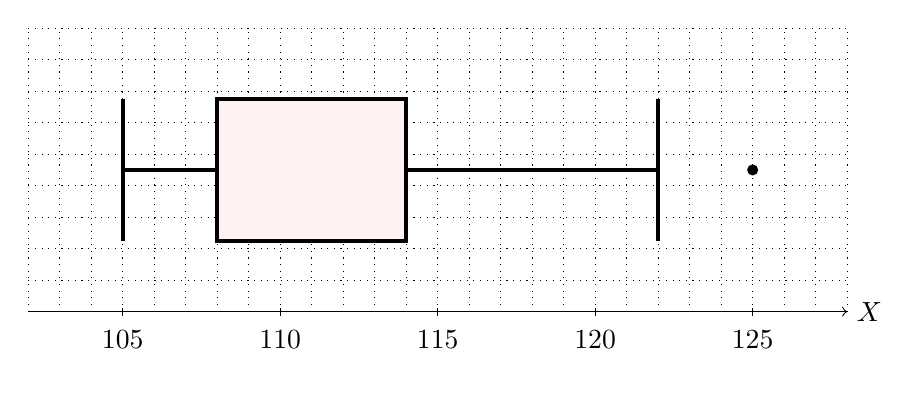
\begin{tikzpicture}[x=0.4cm,y=0.9cm]
         \draw[step=0.4cm,,dotted,color=black] (102,0) grid (128,4);
		\draw[->] (102,0) -- (128,0) node[right] {$X$} ;
		\foreach \X in {105,110,115,120,125} {
			\draw (\X,0.05cm) -- (\X,-0.05cm) node[below] {$\X\strut$};}
		\draw[ultra thick][fill=red!5] (108,1) rectangle (114,3);


		\draw[ultra thick] (105,1) -- (105,3);
		\draw[ultra thick] (105,2) -- (108,2);
		\draw[ultra thick] (114,2) -- (122,2);
		\draw[ultra thick] (122,1) -- (122,3);
        \node[circle, fill=black, inner sep=0pt, minimum size=4pt] at (125,2) {};
			\end{tikzpicture}\\
	\end{center}

\begin{solution}
    Il manque la ligne de la médiane dans le diagramme en boîte. Les 21 données ordonnées donnent une médiane égale à la 11\textsuperscript{e} valeur, soit $\tilde{x}=111$. Il faut donc tracer un trait vertical à $x=111$ à l'intérieur de la boîte.

    On vérifie les autres éléments:
    \begin{itemize}
        \item $Q_1 = (x_{(5)}+x_{(6)})/2=(108+108)/2=108$ \checkmark
        \item $Q_3 = (x_{(16)}+x_{(17)})/2=(114+114)/2=114$ \checkmark
        \item $\text{IQR}=Q_3 - Q_1 = 6$
        \item Barrière supérieure: $Q_3+1{,}5\times\text{IQR}=114+9=123$
        \item La valeur $125 > 123$ est une valeur aberrante, correctement représentée par un point. \checkmark
        \item La moustache supérieure s'arrête à $122$, la plus grande valeur non aberrante. \checkmark
        \item La moustache inférieure s'arrête à $105$, la plus petite valeur (non aberrante car $105 > 108-9=99$). \checkmark
    \end{itemize}
\end{solution}

    \pageblanche

    \question Soit $X_1,\hdots,X_5$ un échantillon de taille $n=5$ provenant d'une variable aléatoire de fonction de répartition $F_X$, d'espérance $\mu$ et de variance $\sigma^2$.

    Pour estimer $\mu$, nous voulons comparer la performance de deux estimateurs:

    \begin{align*}
        \hat{\mu}_1=\overline{X}, & & \hat{\mu}_2=0{,}1X_1+0{,}2X_2+0{,}3X_3+0{,}2X_4+0{,}1X_5.
    \end{align*}

    \begin{parts}
        \part[5] Lequel des deux estimateurs a la plus faible variance?
\begin{solution}
    \begin{align*}
        V(\hat{\mu}_1)&=V(\overline{X})\\
        &=\frac{\sigma^2}{5}=0{,}2\sigma^2
    \end{align*}
    \begin{align*}
        V(\hat{\mu}_2)&=V(0{,}1X_1+0{,}2X_2+0{,}3X_3+0{,}2X_4+0{,}1X_5)\\
        &=0{,}1^2V(X_1)+0{,}2^2V(X_2)+0{,}3^2V(X_3)+0{,}2^2V(X_4)+0{,}1^2V(X_5)\\
        &=(0{,}01+0{,}04+0{,}09+0{,}04+0{,}01)\sigma^2\\
        &=0{,}19\sigma^2
    \end{align*}

    Donc $V(\hat{\mu}_2) = 0{,}19\sigma^2 < V(\hat{\mu}_1) = 0{,}2\sigma^2$.
\end{solution}
        \vspace{8cm}
        \part[7] On sait que $biais(\hat{\mu}_2,\mu)=-0{,}1\mu$. En supposant que $\sigma^2=1$, pour quelles valeurs de $\mu$ a-t-on que l'estimateur $\hat{\mu}_2$ est meilleur que $\hat{\mu}_1$ au niveau du MSE?

        \begin{solution}
            \begin{align*}
                MSE(\hat{\mu}_1,\mu)&=\frac{\sigma^2}{5}\\
                &= 0{,}2
            \end{align*}

                        \begin{align*}
                MSE(\hat{\mu}_2,\mu)&=(-0{,}1\mu)^2+0{,}19\sigma^2\\
                         &= 0{,}01\mu^2+0{,}19
            \end{align*}
            On cherche les valeurs de $\mu$ pour que $MSE(\hat{\mu}_2,\mu)<MSE(\hat{\mu}_1,\mu)$.
                      \begin{align*}
                MSE(\hat{\mu}_2,\mu)&<MSE(\hat{\mu}_1,\mu)\\
                0{,}01\mu^2+0{,}19&<0{,}2\\
                0{,}01\mu^2 &< 0{,}01\\
                \mu^2 &< 1\\
                |\mu| &< 1
            \end{align*}
            
        \end{solution}
    \end{parts}

    \pageblanche

    \question[8] Soit $X_1,\hdots,X_{81}$, des variables aléatoires provenant d'une loi normale d'espérance $\mu=0$ et de variance $\sigma^2=25$. Quelle est la probabilité que $\displaystyle\left|\frac{\overline{X}}{S}\right|$ soit plus grand que $0{,}22$, où $S$ est l'écart-type échantillonnal?

    \begin{solution}
        \begin{align*}
            P\left(\left|\frac{\overline{X}}{S}\right|>0{,}22\right)&=P\left(\left|\frac{\overline{X}}{S/\sqrt{81}}\right|>0{,}22\times 9\right)\\
            &= P\left(\left|t_{80}\right|>1{,}98\right)\\
            &= 2\times P\left(t_{80}>1{,}98\right)\\
            &=2\times 0{,}025\\
            &=0{,}05
        \end{align*}
    \end{solution}

    \pageblanche

    \question Soit $X_1,\hdots, X_{100}$, des variables aléatoires indépendantes et identiquement distribuées selon une loi normale d'espérance $\mu$ et de variance $\sigma^2 = 400$. 
Nous désirons construire un intervalle de confiance approprié de niveau $90\%$ pour $\mu$. Nous notons cet intervalle $[C_1;C_2]$.
\begin{parts}
    \part[3] Que vaut $\mathbb{E}[C_2]$?

    \begin{solution}
        Puisque $\sigma^2 = 400$ est connu et que les $X_i$ suivent une loi normale, l'intervalle de confiance à 90\% est:
        $$\left[\bar{X}-z_{0{,}05}\frac{\sigma}{\sqrt{n}}\;;\;\bar{X}+z_{0{,}05}\frac{\sigma}{\sqrt{n}}\right]=\left[\bar{X}-1{,}645\times\frac{20}{10}\;;\;\bar{X}+1{,}645\times\frac{20}{10}\right]$$
        Donc $C_1=\bar{X}-3{,}29$ et $C_2=\bar{X}+3{,}29$.
        \begin{align*}
            E(C_2)&=E(\bar{X}+3{,}29)\\
            &= E(\bar{X})+3{,}29\\
            &= \mu + 3{,}29
        \end{align*}
    \end{solution}
    \vspace{7cm}
    \part[3] Que vaut $\text{Var}[C_2]$?

    \begin{solution}
        \begin{align*}
            \text{Var}(C_2)&=\text{Var}(\bar{X}+3{,}29)\\
            &= \text{Var}(\bar{X})\\
            &= \frac{\sigma^2}{n}=\frac{400}{100}=4
        \end{align*}
    \end{solution}
    \vspace{7cm}

    \part[4] Quelle est la probabilité que $C_2$ soit inférieure ou égale à $\mu$? 

    \begin{solution}
        \begin{align*}
            P(C_2\leq \mu)&=P(\bar{X}+3{,}29\leq \mu)\\
            &= P\left(\frac{\bar{X}-\mu}{\sigma/\sqrt{n}}\leq \frac{-3{,}29}{20/10}\right)\\
            &= P(Z\leq -1{,}645)\\
            &= 0{,}05
        \end{align*}
    \end{solution}

    \vspace{8cm}


\end{parts}
\end{questions}

\end{document} 
